\documentclass[11pt]{article}
\usepackage[margin=1in]{geometry}
\usepackage{amsmath,amssymb,mathtools,mathrsfs}
\usepackage{tikz}
\usetikzlibrary{decorations.pathmorphing,decorations.pathreplacing,arrows.meta,patterns}
\definecolor{steelblue}{RGB}{70,130,180}
\definecolor{crimson}{RGB}{220,20,60}
\usepackage{graphicx}
\usepackage{xcolor}
\usepackage{hyperref}
\hypersetup{colorlinks=true,linkcolor=blue!60!black,urlcolor=blue!60!black}

\newcommand{\Srel}{S^{\mathrm{rel}}}

\title{\textbf{Supplementary Material:\\ Relative Entropy on the \mbox{Nariai} Horizon}\\[4pt]
\large Diagrams, numerical figures, and reproducibility notes}
\author{Brent S. Hartshorn}

\begin{document}
\maketitle

\noindent
This supplement accompanies the main paper. Section~\ref{sec:geo} illustrates the geometric constructions (the \mbox{Nariai} limit, the bifurcate Killing horizon); Section~\ref{sec:ent} illustrates the entropy results (the ledger equation, the zero-sum interference theorem); Section~\ref{sec:num} presents the numerical figures generated by the scripts in this repository. Every figure is reproducible with \texttt{make}.
\newline
\url{https://github.com/brentharts/NariaiRelativeEntropy}

%=====================================================================
\section{Geometry}
\label{sec:geo}

\subsection{The degenerate limit of Schwarzschild--de Sitter}

The metric function $f(r) = 1 - 2M/r - \Lambda r^2/3$ has two positive roots for $0 < 9\Lambda M^2 < 1$: the black-hole horizon $r_b$ and the cosmological horizon $r_c$. As $9\Lambda M^2 \to 1$ the roots merge at $r_\star = 1/\sqrt{\Lambda}$. In units $\Lambda = 1$:

\begin{center}
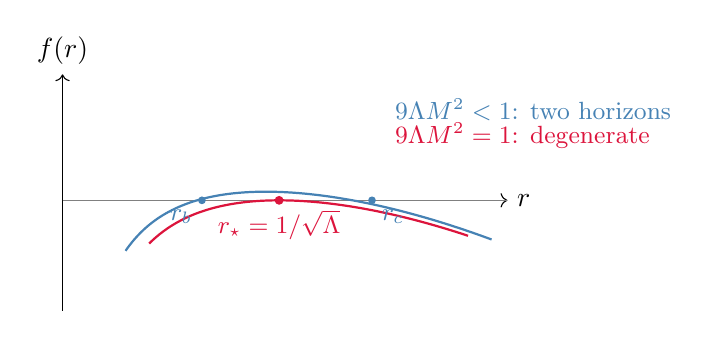
\begin{tikzpicture}[scale=1.0]
  % axes
  \draw[->] (0.25,0) -- (5.9,0) node[right] {$r$};
  \draw[->] (0.25,-1.4) -- (0.25,1.6) node[above] {$f(r)$};
  \draw[gray,very thin] (0.25,0) -- (5.9,0);
  % nondegenerate: M = 0.28  (roots ~ 0.66 and ~ 1.30 scaled by x-unit 3)
  \draw[thick,steelblue,domain=1.05:5.7,samples=120,variable=\x]
    plot ({\x},{ 1 - 2*0.28/(\x/3) - (\x/3)*(\x/3)/3 });
  % degenerate: M = 1/3
  \draw[thick,crimson,domain=1.35:5.4,samples=120,variable=\x]
    plot ({\x},{ 1 - 2*0.3333/(\x/3) - (\x/3)*(\x/3)/3 });
  % markers
  \node[steelblue,anchor=west] at (4.35,1.15) {\small $9\Lambda M^2 < 1$: two horizons};
  \node[crimson,anchor=west]  at (4.35,0.82) {\small $9\Lambda M^2 = 1$: degenerate};
  \fill[crimson] (3.0,0) circle (1.6pt) node[below,crimson] {\small $r_\star = 1/\sqrt{\Lambda}$};
  \fill[steelblue] (2.02,0) circle (1.4pt) node[below left,steelblue] {\small $r_b$};
  \fill[steelblue] (4.18,0) circle (1.4pt) node[below right,steelblue] {\small $r_c$};
\end{tikzpicture}
\end{center}

\noindent
The blue curve crosses zero twice: two horizons, two unequal surface gravities $\kappa_{b,c} = \tfrac12 |f'(r_{b,c})|$, two temperatures, and (by the Kay--Wald obstruction) \emph{no} globally regular equilibrium state. The red curve touches zero tangentially: one degenerate horizon, and --- after the Ginsparg--Perry rescaling of time --- a single surface gravity $\kappa = \sqrt{\Lambda}$ and a genuine global KMS state. Degeneracy is the feature, not the bug.

\subsection{The \mbox{Nariai} bifurcate Killing horizon}

In the limit the geometry becomes $dS_2 \times S^2$: a two-dimensional de~Sitter factor, every point of which carries a round two-sphere of radius $1/\sqrt{\Lambda}$. The Penrose diagram of the $dS_2$ factor is a square; the bifurcate Killing horizon is the pair of diagonals.

\begin{center}
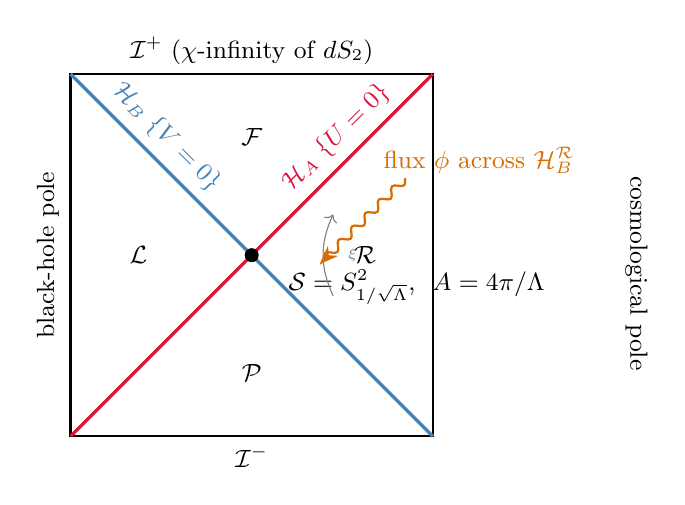
\begin{tikzpicture}[scale=1.15]
  % Penrose square
  \draw[thick] (-2,-2) rectangle (2,2);
  \node[above] at (0,2) {\small $\mathcal{I}^+$ ($\chi$-infinity of $dS_2$)};
  \node[below] at (0,-2) {\small $\mathcal{I}^-$};
  % diagonals = horizons
  \draw[very thick,crimson]  (-2,-2) -- (2,2) node[pos=0.78,above,sloped] {\small $\mathcal{H}_A\ \{U=0\}$};
  \draw[very thick,steelblue] (-2,2) -- (2,-2) node[pos=0.22,above,sloped] {\small $\mathcal{H}_B\ \{V=0\}$};
  % bifurcation surface
  \fill[black] (0,0) circle (2.2pt);
  \node[anchor=north west] at (0.3,-0.05) {\small $\mathcal{S} = S^2_{1/\sqrt{\Lambda}}$,\ \ $A = 4\pi/\Lambda$};
  % wedges
  \node at (1.25,0) {\small $\mathcal{R}$};
  \node at (-1.25,0) {\small $\mathcal{L}$};
  \node at (0,1.3) {\small $\mathcal{F}$};
  \node at (0,-1.3) {\small $\mathcal{P}$};
  % poles
  \node[rotate=90] at (-2.25,0) {\small black-hole pole};
  \node[rotate=-90] at (4.25,-0.2) {\small cosmological pole};
  % Killing flow arrows in R wedge
  \draw[->,gray] (0.9,-0.45) to[bend left=25] (0.9,0.45);
  \node[gray,anchor=west] at (0.95,0.0) {\tiny $\xi$};
  % coherent flux crossing H_B^R
  \draw[-{Stealth[length=2.4mm]},decorate,decoration={snake,amplitude=.5mm,segment length=2.4mm},thick,orange!85!black]
    (1.7,0.85) -- (0.75,-0.1);
  \node[orange!85!black,anchor=west] at (1.35,1.05) {\small flux $\phi$ across $\mathcal{H}_B^{\mathcal{R}}$};
\end{tikzpicture}
\end{center}

\noindent
Every point of the square is a two-sphere; the bifurcation surface $\mathcal{S}$ at the center is \emph{compact}, with total area $4\pi/\Lambda$ --- the finiteness that removes the infinite-area caveat of the local Rindler construction. The left and right edges of the square are the two ``poles'' into which the degenerate horizon splits under perturbation: the branch structure of the (anti-)evaporation instability lives on this diagram. The modular flow of the wedge algebra $(\mathscr{N}_{\mathcal{R}}, \Omega_0)$ is the geometric Killing flow $\xi$ shown in the right wedge.

%=====================================================================
\section{Entropy}
\label{sec:ent}

\subsection{The ledger equation}

On \mbox{Nariai} the identification $\Srel = \delta A/4$ relates \emph{finite} quantities. The total geometric entropy of the perturbed bifurcation surface splits into a state-independent extremal capacity and a state-dependent record of realized distinctions:

\begin{center}
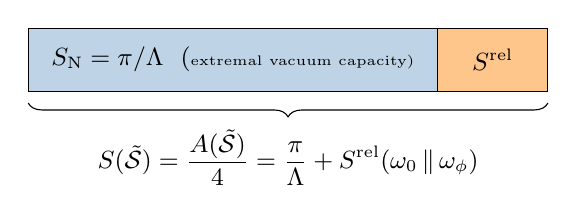
\begin{tikzpicture}[scale=1.0]
  % vacuum bar
  \fill[steelblue!35] (0,0) rectangle (5.2,0.8);
  \draw (0,0) rectangle (5.2,0.8);
  \node at (2.6,0.4) {\small $S_{\mathrm{N}} = \pi/\Lambda$\ \ (\tiny extremal vacuum capacity)};
  % excitation increment
  \fill[orange!45] (5.2,0) rectangle (6.6,0.8);
  \draw (5.2,0) rectangle (6.6,0.8);
  \node at (5.9,0.4) {\small $\Srel$};
  % total brace
  \draw[decorate,decoration={brace,amplitude=5pt,mirror},yshift=-2pt]
    (0,-0.08) -- (6.6,-0.08) node[midway,below=6pt]
    {\small $S(\tilde{\mathcal{S}}) = \dfrac{A(\tilde{\mathcal{S}})}{4} = \dfrac{\pi}{\Lambda} + \Srel(\omega_0\,\|\,\omega_\phi)$};
\end{tikzpicture}
\end{center}

\noindent
The increment is the Araki--Uhlmann relative entropy: the information distinguishing the realized state from the counterfactual vacuum --- an entropy of \emph{events relative to non-events}, recorded in area.

\subsection{The zero-sum interference theorem}

The central exact result of Appendix~B of the main paper: with $U = -\kappa^{-1}e^{-\kappa u}$, the modular weight is precisely the boost Jacobian, $(-U)\,dU = \kappa^{-1}\,du$, so the interference functional
\[
I_2 = \int (-U)\,\big(\partial_U\chi\big)^2\, dU\, d\mathrm{vol}_{\mathcal{S}}
    = \frac{1}{\kappa}\int \big(\partial_u\chi\big)^2\, du \, d\mathrm{vol}_{\mathcal{S}}
\]
is the zero-total-boost-frequency Fourier component of $(\partial_u\chi)^2$ --- which \emph{vanishes identically} for boost-positive-frequency packets. Schematically:

\begin{center}
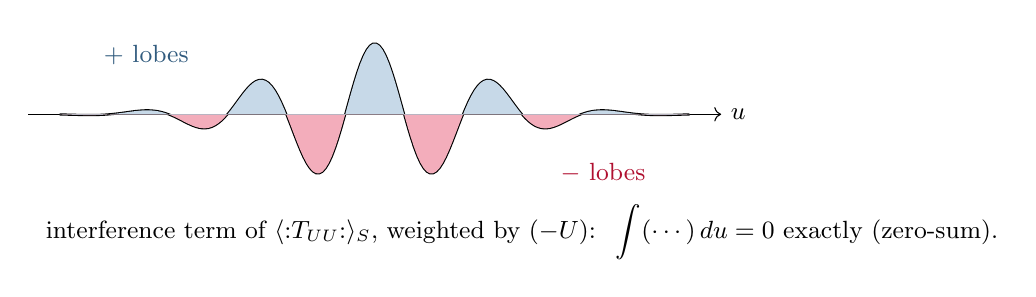
\begin{tikzpicture}[scale=1.0]
  \draw[->] (-4.4,0) -- (4.4,0) node[right] {\small $u$};
  % interference term: oscillatory, equal shaded areas
  \draw[thick,domain=-4:4,samples=200,variable=\x]
    plot ({\x},{ 0.9*exp(-\x*\x/3.0)*cos(deg(4.2*\x)) });
  \fill[crimson!40,domain=-0.375:0.375,variable=\x]
    (-0.375,0) -- plot ({\x},{ -0.9*exp(-\x*\x/3.0)*abs(cos(deg(4.2*\x)))*0 }) -- (0.375,0) -- cycle;
  % shade negative lobes approximately
  \begin{scope}
    \clip (-4,-1.1) rectangle (4,0);
    \fill[crimson!35,domain=-4:4,samples=200,variable=\x]
      plot ({\x},{ 0.9*exp(-\x*\x/3.0)*cos(deg(4.2*\x)) }) -- (4,0) -- (-4,0) -- cycle;
  \end{scope}
  \begin{scope}
    \clip (-4,0) rectangle (4,1.1);
    \fill[steelblue!30,domain=-4:4,samples=200,variable=\x]
      plot ({\x},{ 0.9*exp(-\x*\x/3.0)*cos(deg(4.2*\x)) }) -- (4,0) -- (-4,0) -- cycle;
  \end{scope}
  \node[steelblue!70!black] at (-2.9,0.75) {\small $+$ lobes};
  \node[crimson!80!black]   at (2.9,-0.75) {\small $-$ lobes};
  \node[anchor=west] at (-4.3,-1.5) {\small interference term of $\langle{:}T_{UU}{:}\rangle_S$, weighted by $(-U)$:
        \ $\displaystyle\int(\cdots)\,du = 0$ exactly (zero-sum).};
\end{tikzpicture}
\end{center}

\noindent
Consequences: the squeezed relative entropy takes the thermal first-law form $\Srel = \beta\,\Delta E_{\mathrm{boost}}$ with $\beta = 2\pi/\sqrt{\Lambda}$; local negativity windows (the engine of anti-evaporation) exist but are prepaid, unit for unit, by positive flux elsewhere on the same horizon; and the squeeze--shape functional $|I_2|/I_1$ is a binary wedge-locality detector: $0$ for boost-adapted data, $1$ for boost-blind data.

%=====================================================================
\section{Numerical figures}
\label{sec:num}

The three figures below are produced by \texttt{generate\_figures.py}; the quantitative claims of the main paper's Appendix~B are checked by \texttt{appendix\_b\_verification.py}. Both run from the \texttt{Makefile}.

\begin{center}
\includegraphics[width=0.92\textwidth]{figures/fig_flux_windows}
\end{center}
\noindent\textbf{Figure S1.} The squeezed horizon flux in boost time at $(r,\theta) = (0.5, \pi)$. Red regions are the negativity windows $\mathcal{W}$ --- genuine local violations of the classical positivity that drives the coherent-sector selection rule. The modular-weighted total remains positive; the oscillatory (interference) part integrates to zero exactly.

\begin{center}
\includegraphics[width=0.8\textwidth]{figures/fig_dichotomy}
\end{center}
\noindent\textbf{Figure S2.} The squeeze--shape functional $|I_2|/I_1$ as the packet's spectral weight is pushed below zero boost frequency. Boost-adapted packets sit at the exact zero (the vanishing theorem); as negative-frequency content grows, the functional climbs toward the boost-blind value $1$, where no wedge-local squeeze exists at any finite $r$.

\begin{center}
\includegraphics[width=0.8\textwidth]{figures/fig_one_mode}
\end{center}
\noindent\textbf{Figure S3.} One-mode verification of the sum rule $\Srel = \beta\,\Delta E$: relative entropy computed from covariance matrices (points) against the closed form $\beta\,\omega\,\sinh^2\!r\,\coth(\beta\omega/2)$ (curves), for three boost-mode frequencies. Agreement is at machine precision; the $\coth$ factor is the thermal occupancy of the wedge mode.

%=====================================================================
\section*{Reproducibility}
\texttt{make figures} regenerates Figures S1--S3; \texttt{make verify} reruns the numerical checks; \texttt{make} builds this document. Python $\ge 3.10$ with \texttt{numpy} and \texttt{matplotlib}, and a \TeX{} distribution with Ti\emph{k}Z, are the only requirements.

\end{document}
